% 来源：固定1991上海PDF第3页（印刷5-35），第27题。
% 忠实复现A/B/C、a/b/c和C处theta角弧；示意比例不是题设。
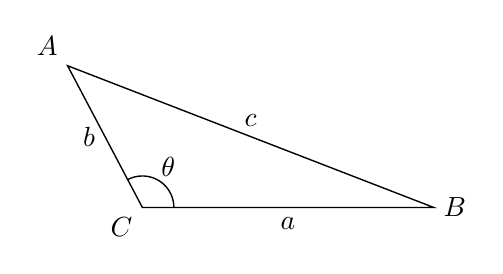
\begin{tikzpicture}[line width=0.5pt,scale=1.0]
  \coordinate (A) at (-0.95,1.8);
  \coordinate (B) at (3.7,0);
  \coordinate (C) at (0,0);
  \draw (A)--node[above] {$c$} (B)--node[below] {$a$} (C)--node[left] {$b$} cycle;
  \draw (0.4,0) arc[start angle=0,end angle=117.82,radius=0.4];
  \node at (0.33,0.52) {$\theta$};
  \node[above left] at (A) {$A$};
  \node[right] at (B) {$B$};
  \node[below left] at (C) {$C$};
\end{tikzpicture}
